% Chapter Template

\chapter{FDTD - Two-Dimensional Scenario} % Main chapter title

\label{Chapter3} % Change X to a consecutive number; for referencing this chapter elsewhere, use \ref{ChapterX}

%----------------------------------------------------------------------------------------
%	SECTION 1
%----------------------------------------------------------------------------------------

\section{Main Section 1}

%-----------------------------------
%	SUBSECTION 1
%-----------------------------------
\subsection{Subsection 1}
%-----------------------------------
%	SUBSECTION 2
%-----------------------------------

\subsection{Subsection 2}
%----------------------------------------------------------------------------------------
%	SECTION 2
%----------------------------------------------------------------------------------------

\section{C++ Implementation}

\begin{minted}[breaklines,frame=single]{c++}
	double L = 5;
	int N = 200;
	int iterNum = 800;
	double deltaX = L / N;
	double deltaY = L / N;
	double deltaZ = L / N;
	double deltaT = (deltaZ * sqrt(permitivity*permeability)  * (1/sqrt(2))); // 1/C * 1/sqrt2 * deltaZ
	
	// variables needed for Gaussian Pulse excitation
	double eps = 1e-3;
	double Teps = 50 * deltaT;
	double beta = -(pow((2/Teps), 2) * log(eps));
	
	
	vector<vector<double>> Ex(N, vector<double> (N, 0));
	vector<vector<double>> Ey(N, vector<double> (N, 0));
	vector<vector<double>> Hz(N, vector<double> (N, 0));
	
	const string filePath = "./Out/";
	
	void writeEDataToCsvFile(string filename, vector<vector<double>> Ex, vector<vector<double>> Ey){
		
		//	"x","y",Ex,Ey
		//	0,0,Ex[x,y],Ey[x,y]
		
		ofstream csvFile(filename);
		csvFile << "x,y,z,Ex,Ey\n";
		
		for (int x = 0; x < Ex[0].size(); x++) {
			for (int y = 0; y < Ex[x].size(); y++) {
				csvFile << to_string(x) + "," + to_string(y) + ",0," + to_string(Ex[x][y]) + "," + to_string(Ey[x][y]) + "\n";
			}
		}
		
		csvFile.close();
	}
	
	void writeHDataToCsvFile(string filename, vector<vector<double>> Hz){
		
		//	"x","y",Hz
		//	0,0,Hz[x,y]
		
		ofstream csvFile(filename);
		csvFile << "x,y,z,Hz\n";
		
		for (int x = 0; x < Hz[0].size(); x++) {
			for (int y = 0; y < Ex[x].size(); y++) {
				csvFile << to_string(x) + "," + to_string(y) + ",0," + to_string(Hz[x][y]) + "\n";
			}
		}
		
		csvFile.close();
	}
	
	int main()
	{
		for(int i = 0; i < iterNum; i++) {
			
			double t = i * deltaT;
			double gamma = Teps / 2;
			
			// reducing the magnitude since in free space
			Hz[99][99] = exp(-(beta * pow((t - gamma), 2))) * 10e-4;  //TO-DO: Gaussian excitation, alpha = 1, Teps = 50*deltaT, eps = 1e-3, t = i * deltaT
			
			for (int i = 0; i < N-1; i++) {
				for (int j = 1; j < N-2; j++) {
					Ex[i][j] = Ex[i][j] + (deltaT / permitivity / deltaZ) * (Hz[i][j] - Hz[i][j-1]);
				}
			}
			
			for (int i = 1; i < N-2; i++) {
				for (int j = 0; j < N-1; j++) {
					Ey[i][j] = Ey[i][j] - ((deltaT / permitivity / deltaZ) * (Hz[i][j] - Hz[i-1][j]));
				}
			}
			
			writeEDataToCsvFile((filePath + "E/E.csv." + to_string(i)), Ex, Ey);
			
			// loop for values
			for (int i = 0; i < N-1; i++) {
				for (int j = 0; j < N-1; j++) {
					Hz[i][j] = Hz[i][j] - ((deltaT / permeability / deltaZ) * (Ex[i][j] - Ex[i][j+1] + Ey[i+1][j] - Ey[i][j]));
				}
			}
			
			
			writeHDataToCsvFile((filePath + "H/H.csv." + to_string(i)), Hz);
			
		}
	}
\end{minted}


\section{Data Visualization}

\begin{figure}
	\centering
    \begin{subfigure}{.49\textwidth}
    	\centering
    	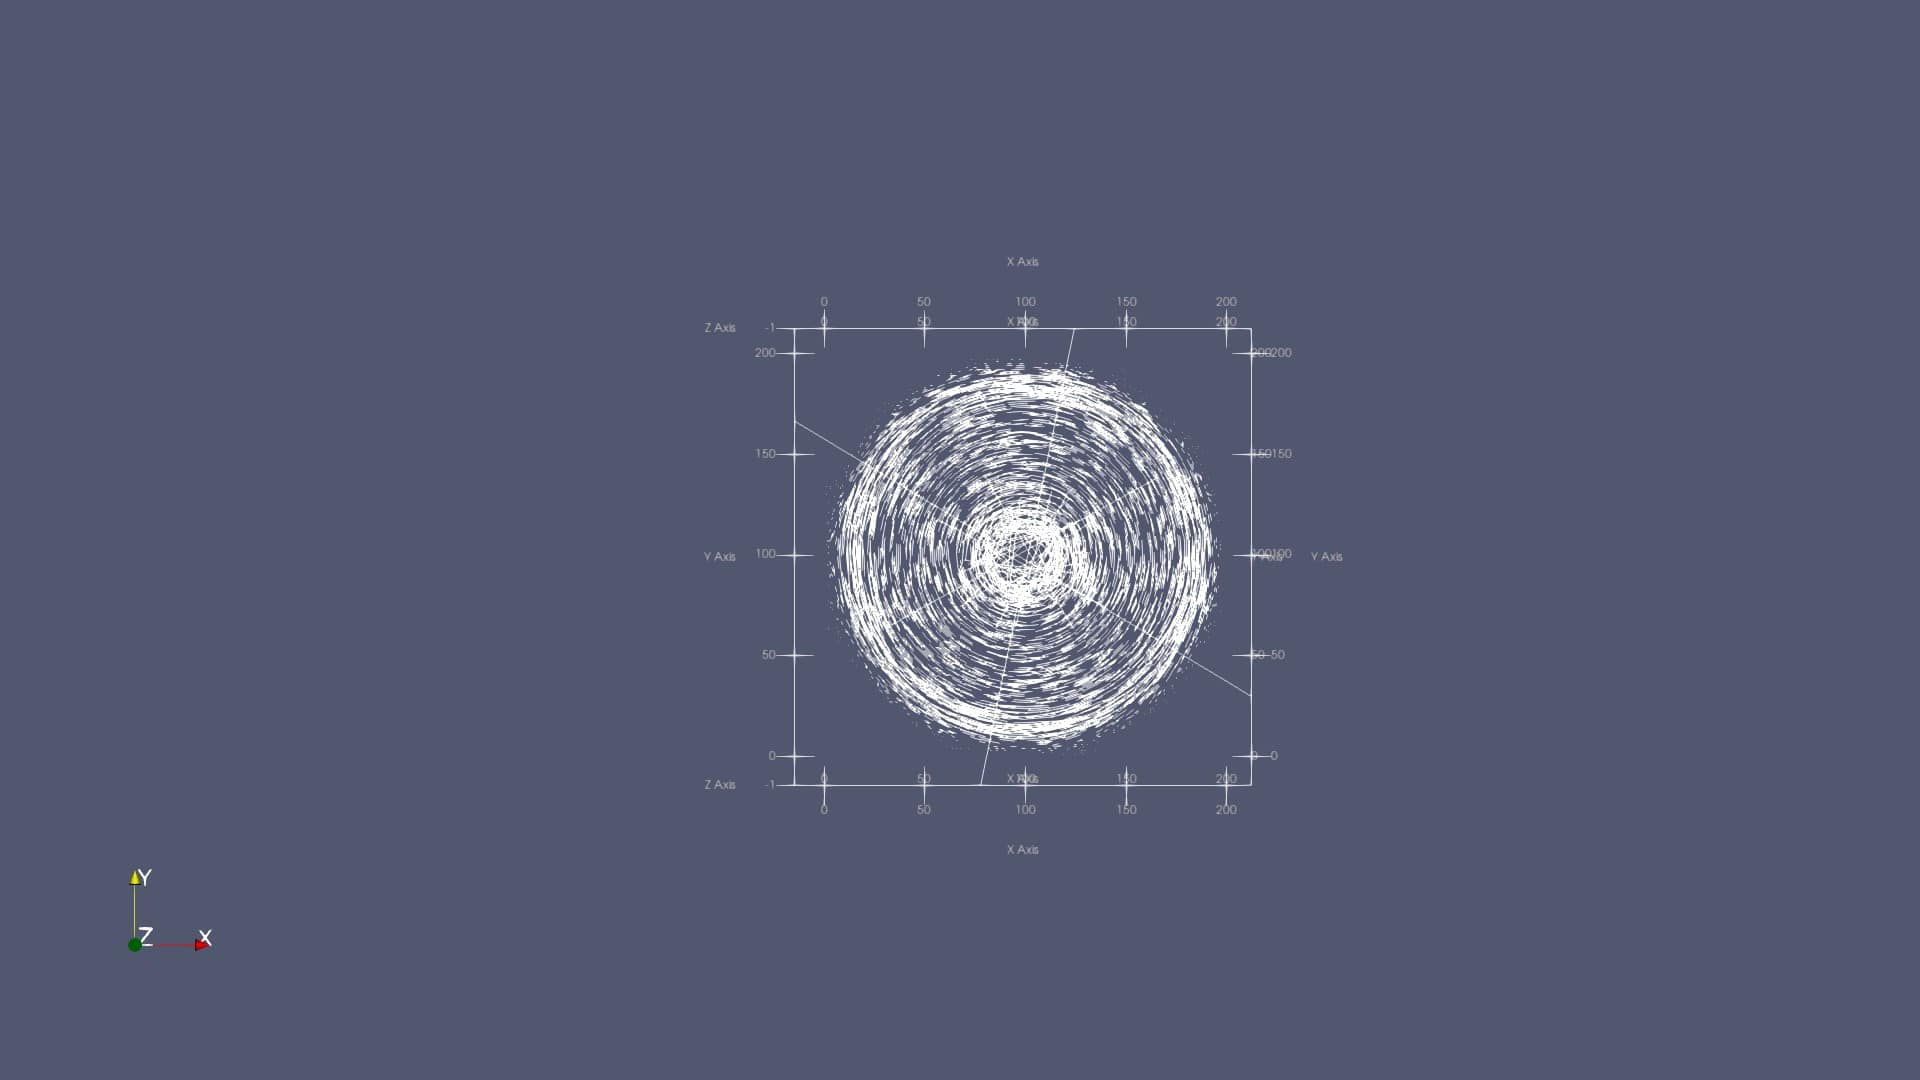
\includegraphics[width=.95\linewidth]{Figures/FDTD2DE1}
    	\caption{t = 200}
    \end{subfigure}
    \begin{subfigure}{.49\textwidth}
    	\centering
    	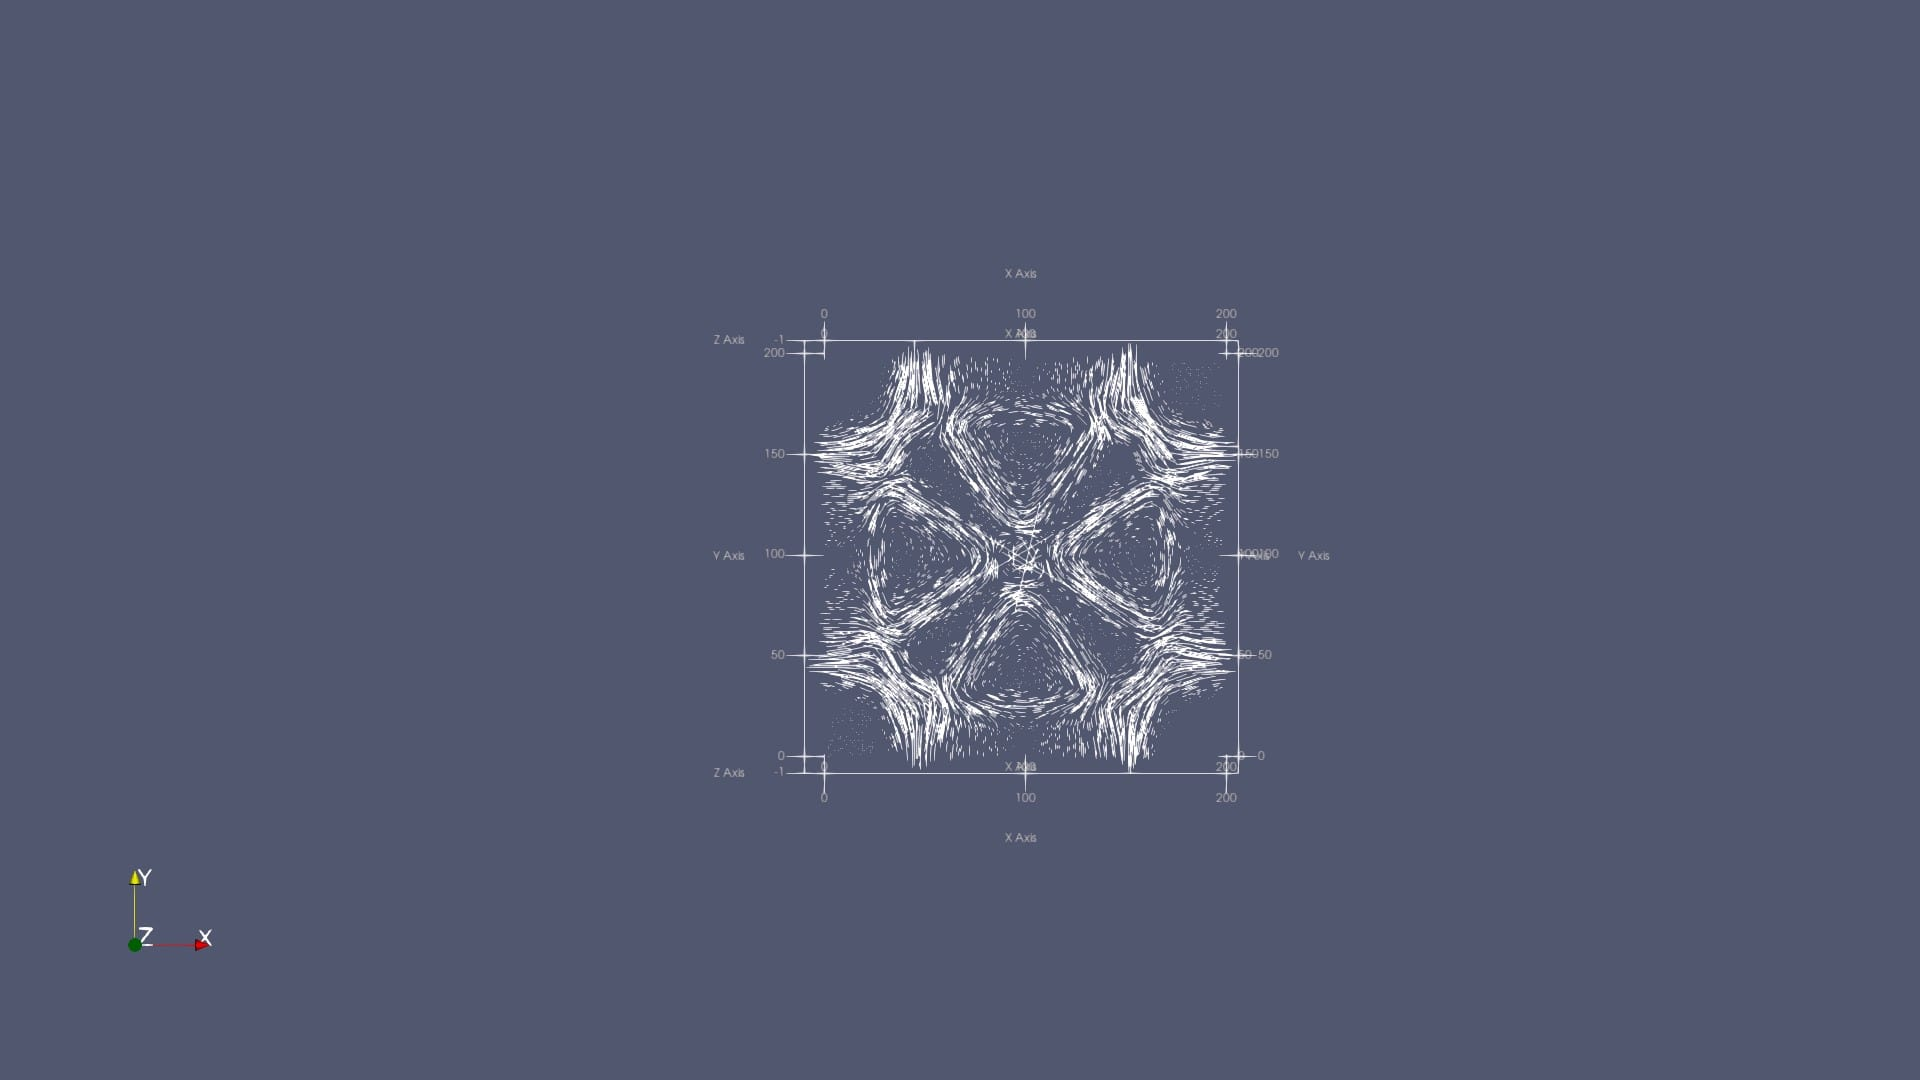
\includegraphics[width=.95\linewidth]{Figures/FDTD2DE2}
    	\caption{t = 400}
    \end{subfigure}
    \begin{subfigure}{.49\textwidth}
    	\centering
    	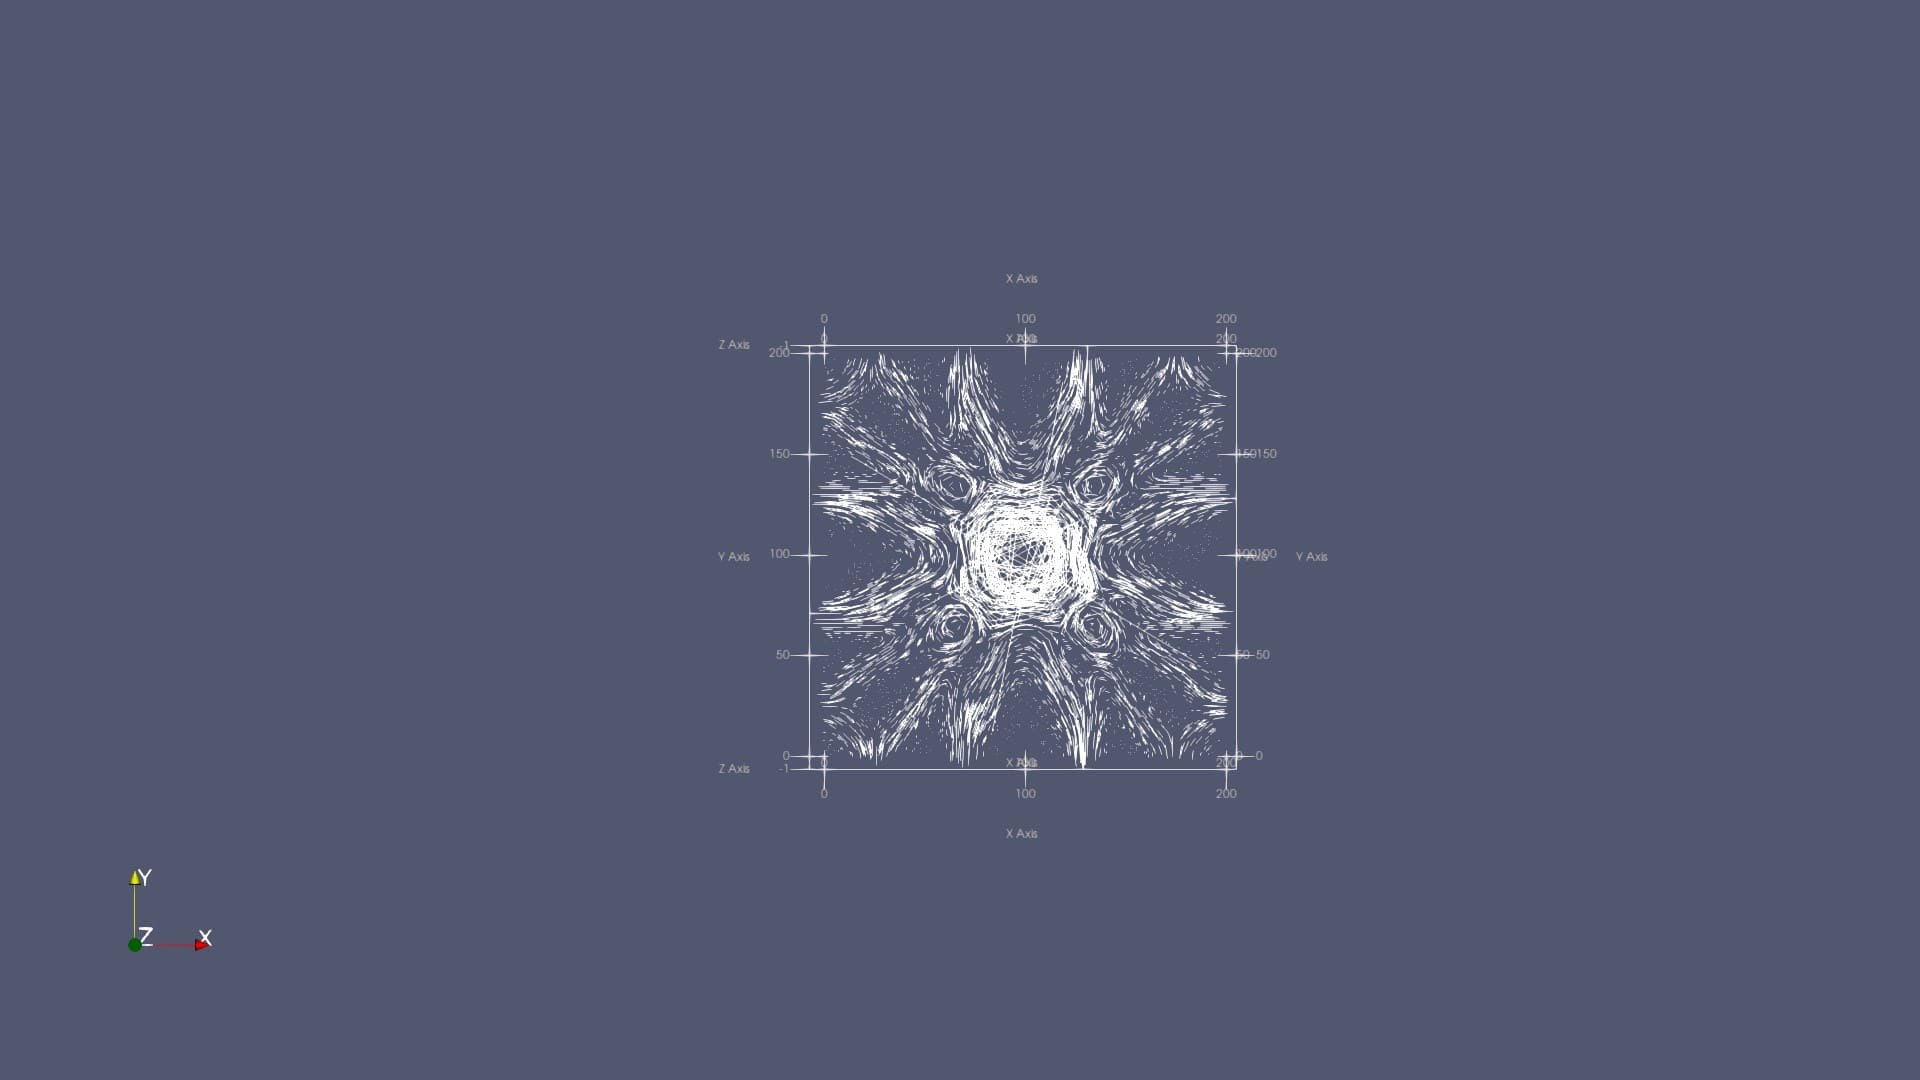
\includegraphics[width=.95\linewidth]{Figures/FDTD2DE3}
    	\caption{t = 600}
    \end{subfigure}
    \begin{subfigure}{.49\textwidth}
    	\centering
    	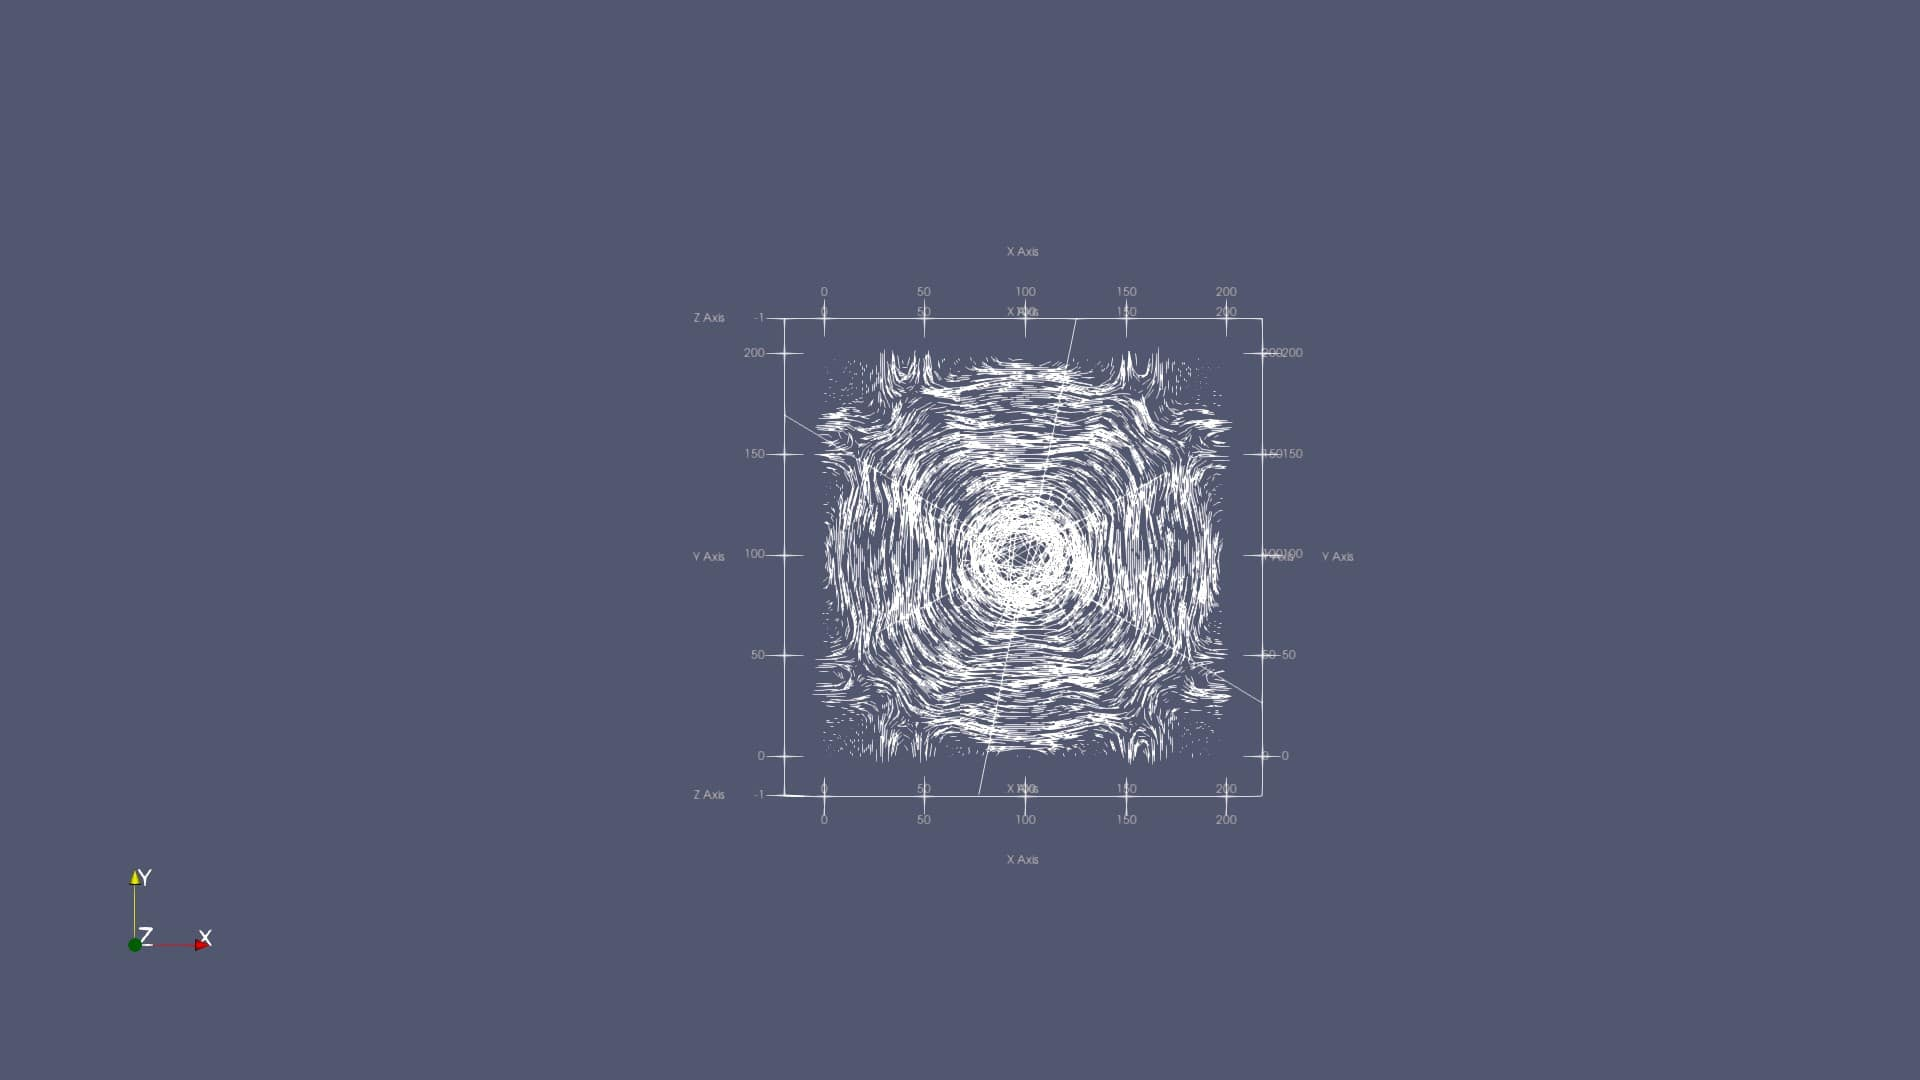
\includegraphics[width=.95\linewidth]{Figures/FDTD2DE4}
    	\caption{t = 800}
    \end{subfigure}
	\decoRule
	\caption[2D Electric Field Simulation]{A simulation of the 2D electric field.}
	\label{fig:FDTD2DE}
\end{figure}

\begin{figure}
	\centering
	\begin{subfigure}{.49\textwidth}
		\centering
		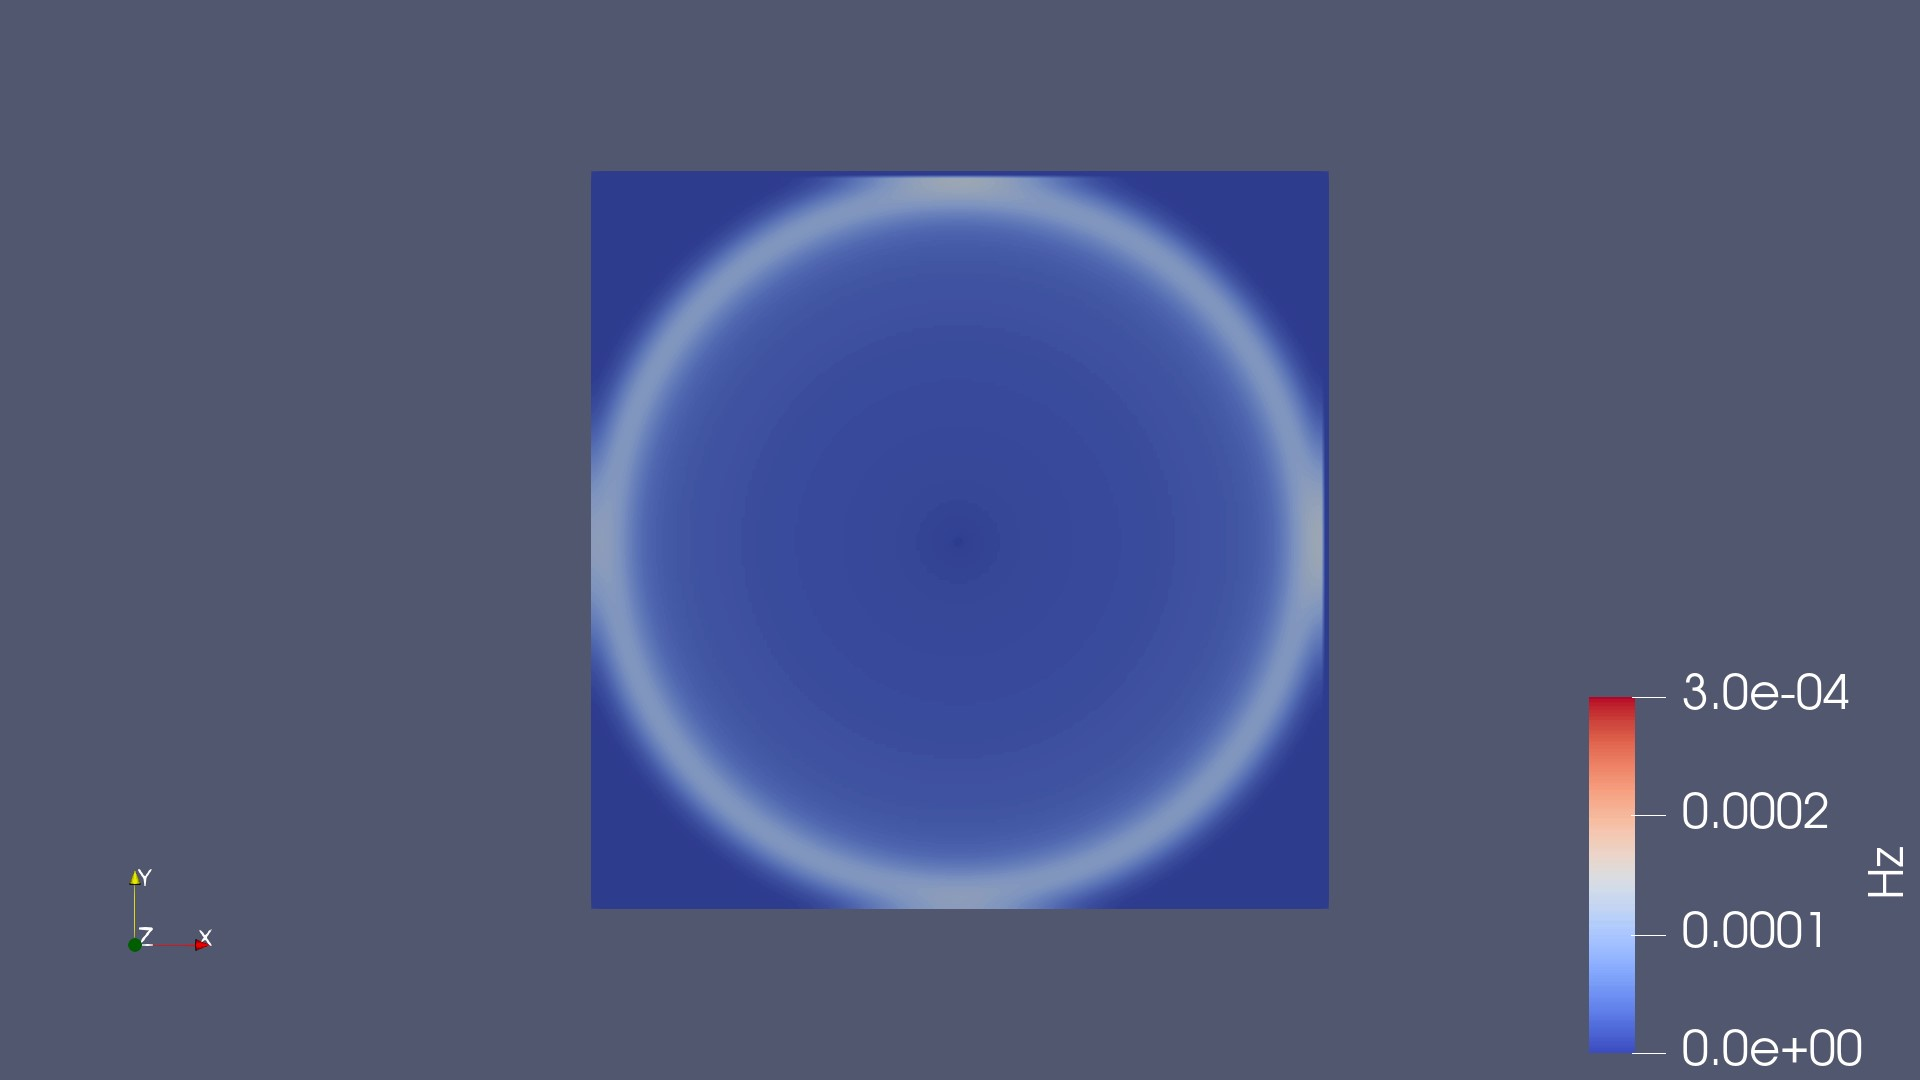
\includegraphics[width=.95\linewidth]{Figures/FDTD2DH1}
		\caption{t = 200}
	\end{subfigure}
	\begin{subfigure}{.49\textwidth}
		\centering
		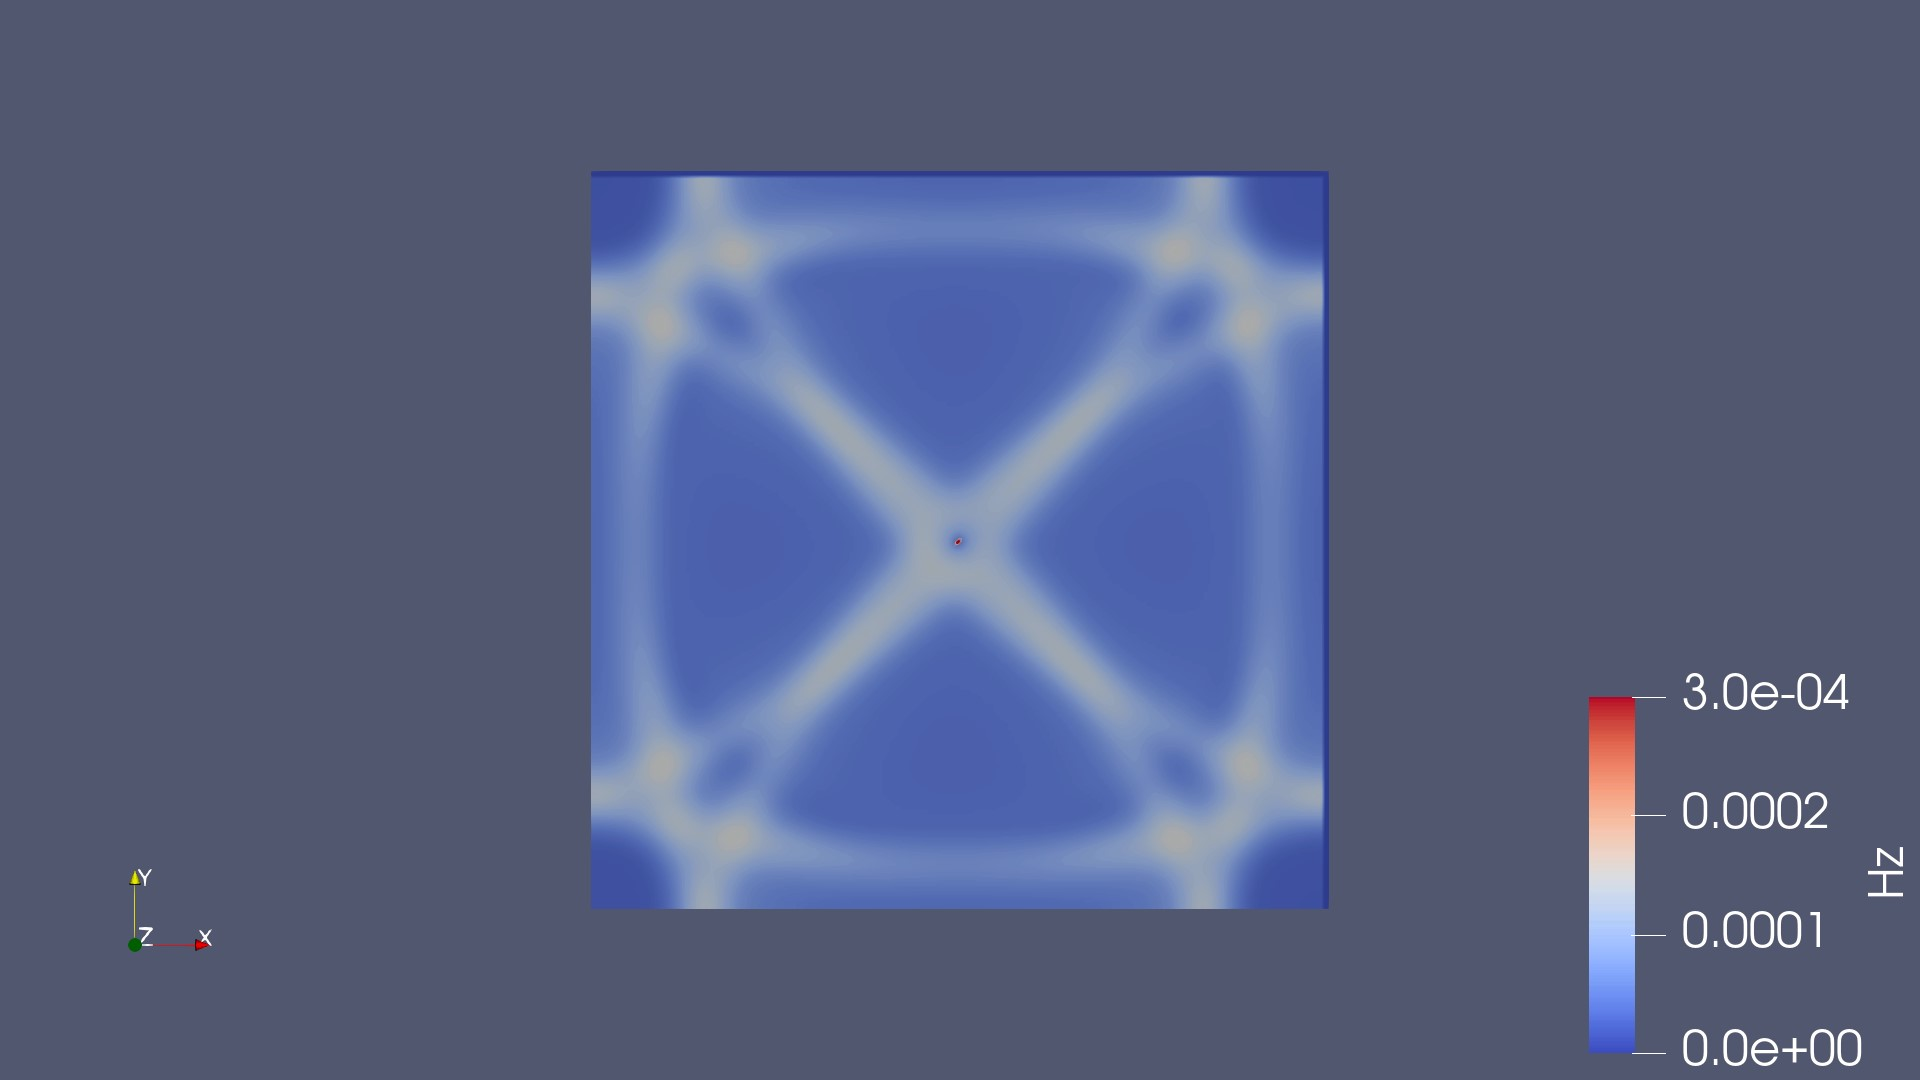
\includegraphics[width=.95\linewidth]{Figures/FDTD2DH2}
		\caption{t = 400}
	\end{subfigure}
	\begin{subfigure}{.49\textwidth}
		\centering
		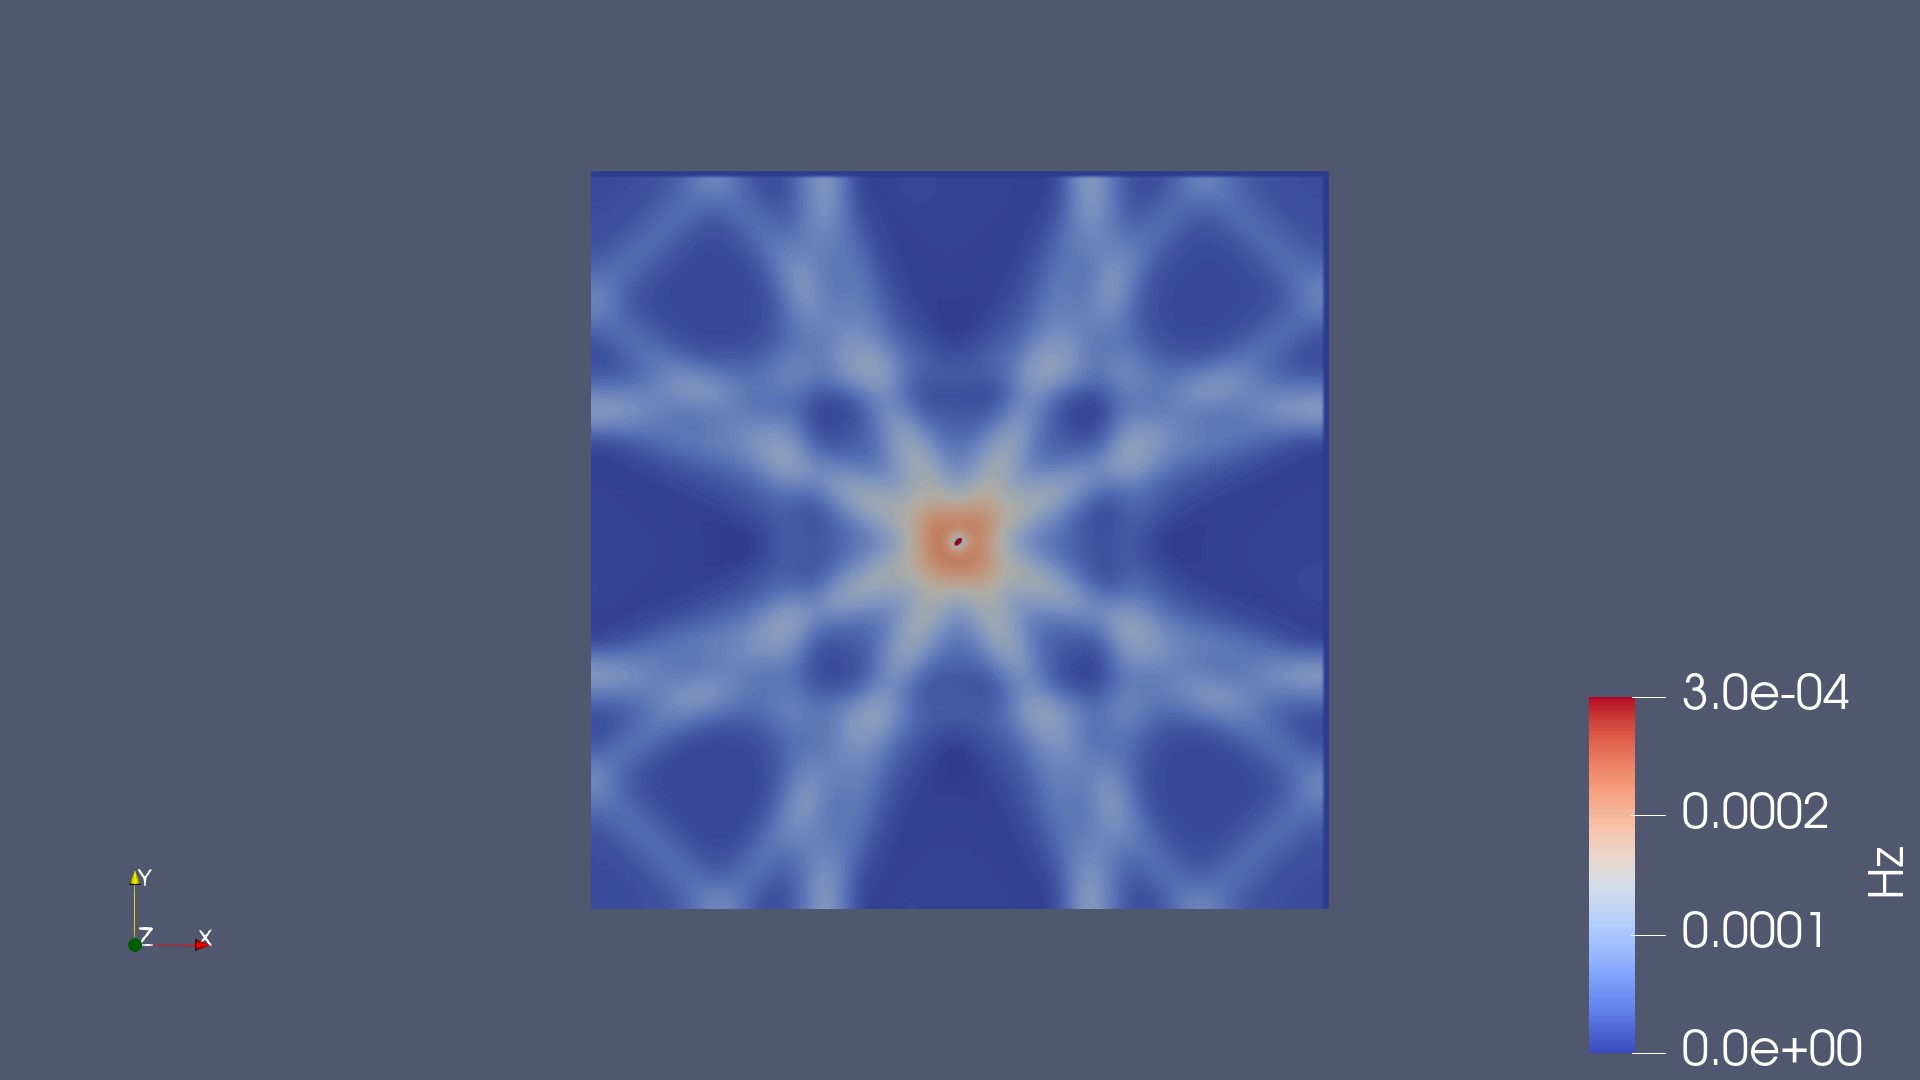
\includegraphics[width=.95\linewidth]{Figures/FDTD2DH3}
		\caption{t = 600}
	\end{subfigure}
	\begin{subfigure}{.49\textwidth}
		\centering
		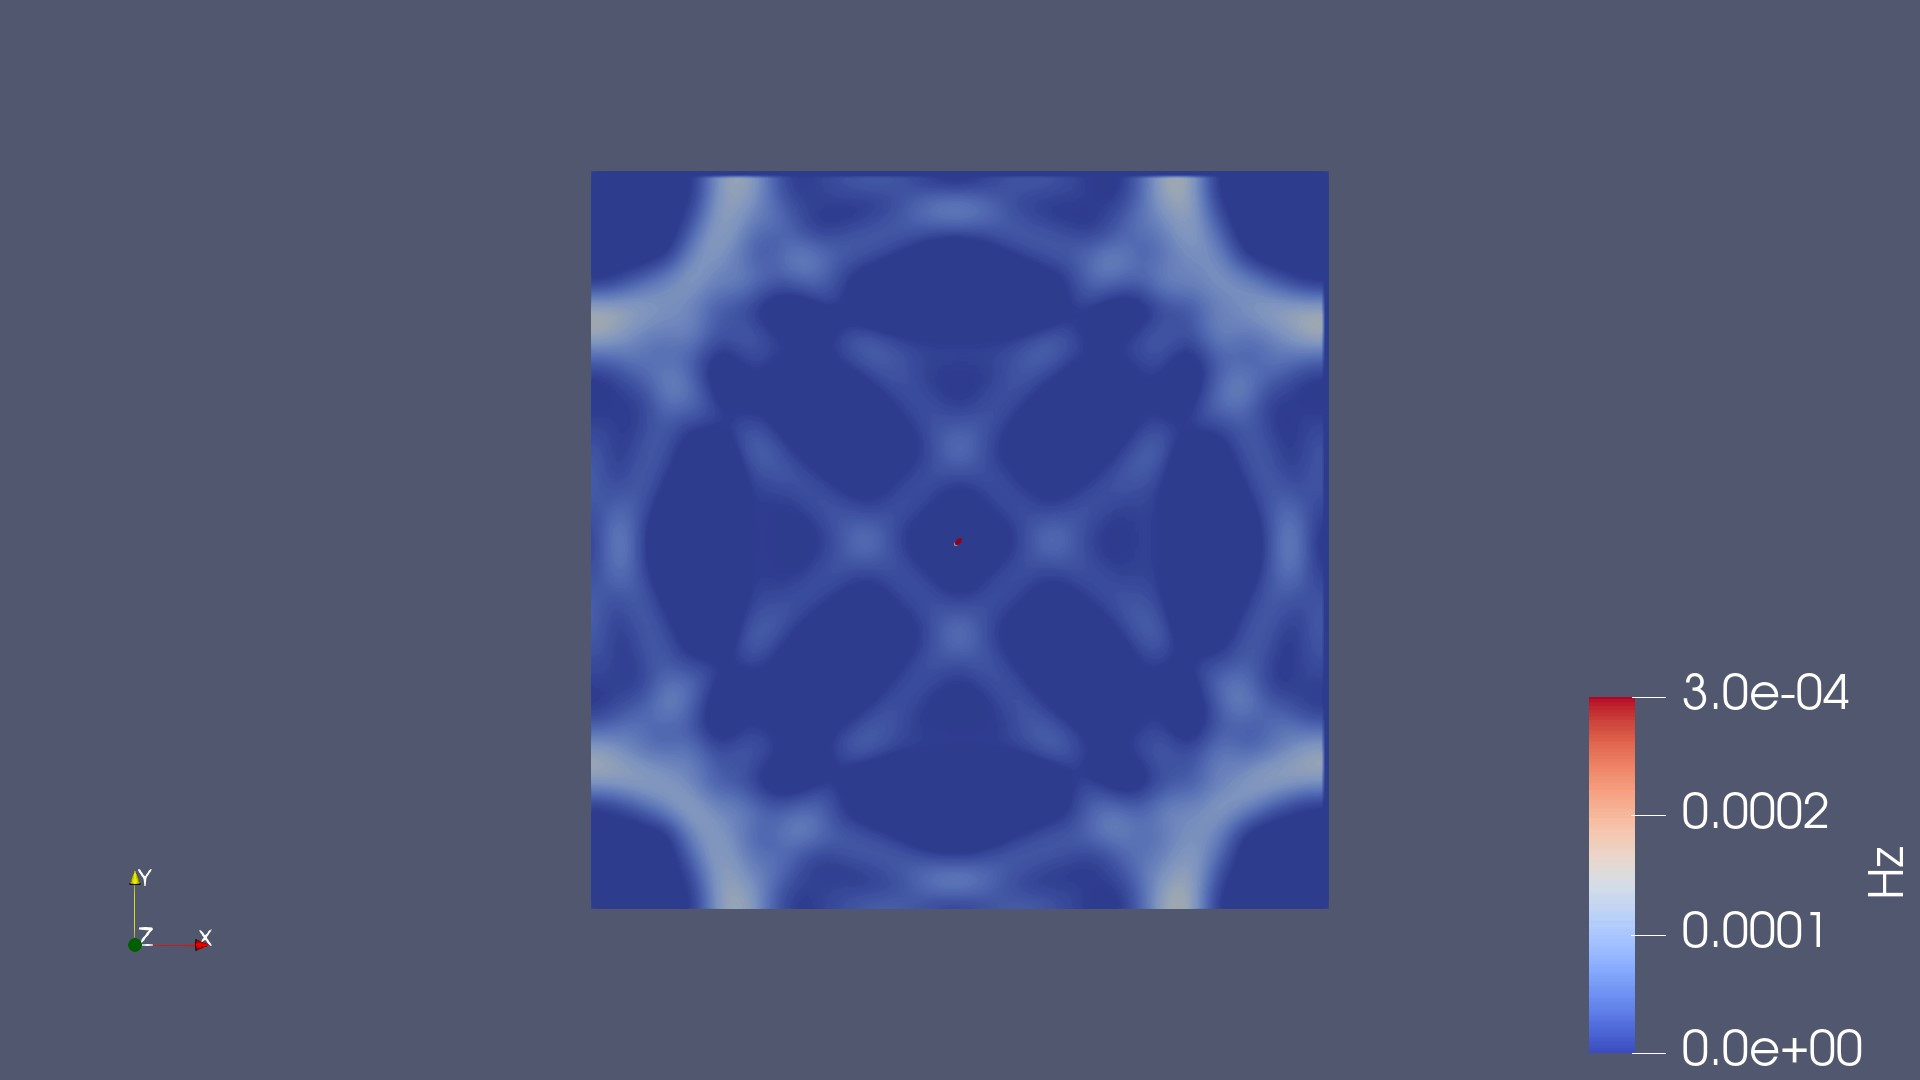
\includegraphics[width=.95\linewidth]{Figures/FDTD2DH4}
		\caption{t = 800}
	\end{subfigure}
	\decoRule
	\caption[2D Magnetic Field Simulation]{A simulation of the 2D magnetic field.}
	\label{fig:FDTD2DH}
\end{figure}